%----------------------------------------------------------------------------
%bb defines the bounding box for the pdf
%viewport defines the area of the pdf used
%in sidewaysfigure the last entry in bb moves the caption toward/away the pic
%in sidewaysfigure the second entry in bb moves the pic toward/away the caption
%----------------------------------------------------------------------------
\begin{figure}
\scalebox{0.8}[0.8]{
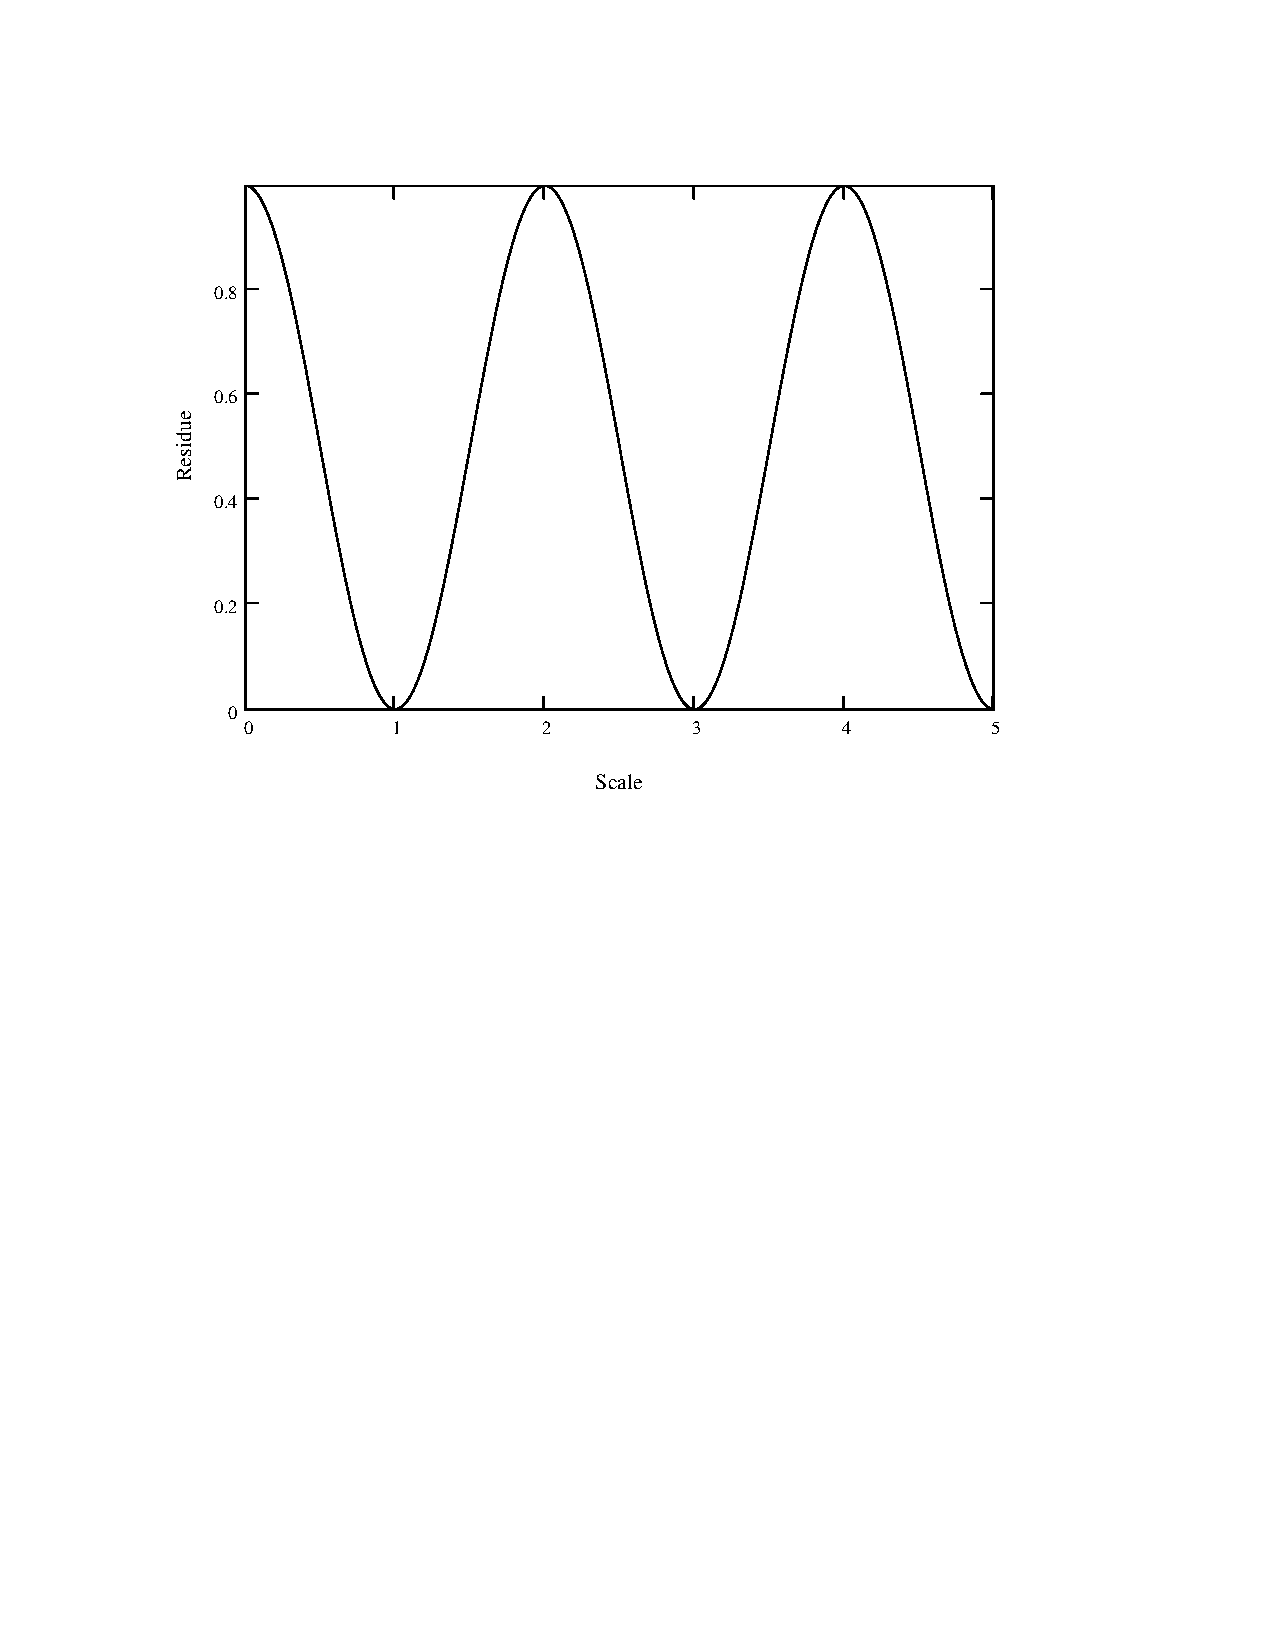
\includegraphics[bb=30 415 489 715]
{scale_three-color/scale_three-color.pdf}
}
\caption[Amplitude ``non-robustness'' of the three color STIRAP]{Amplitude ``non-robustness'' of the three color STIRAP. The optimal solution in Figure \ref{solution three pulses} is allowed to vary in pulse height by the ``scale'' factor (all three pulses are scaled simultaneously) and the resulting residue, as defined by Equation \ref{phi prime} is plotted as a function of the scale.}
\label{scale_three-color}
\end{figure}
%----------------------------------------------------------------------------
